\documentclass[a4j,titlepage]{jarticle}
\usepackage[dvipdfmx]{graphicx}
\usepackage{ascmac}
\usepackage{float}
\usepackage{amssymb}%にやりイコールを使う
\usepackage{multirow}
\usepackage{multicol}
%\usepackage{color}

\begin{document}

\title{2022 年度 3 回生前期学生実験 HW  \\ \bf team02 方式設計仕様書}
% ↓ここに自分の氏名を記入
\author{方式設計仕様書作成者:植田健斗\\
グループメンバー:\\伊藤舜一郎 (学籍番号:1029-32-7548)
\\植田健斗 (学籍番号:1029-32-6498)}
\西暦
\date{提出期限:5月12日18時 提出日: \today} % コンパイル時の日付が自動で挿入される
\maketitle
\newpage

\section{概要}

\section{命令セット・アーキテクチャ}
命令セットアーキテクチャは以下の図\ref{instructionSet}のようになる。

\begin{figure}[H]
    \begin{center}
    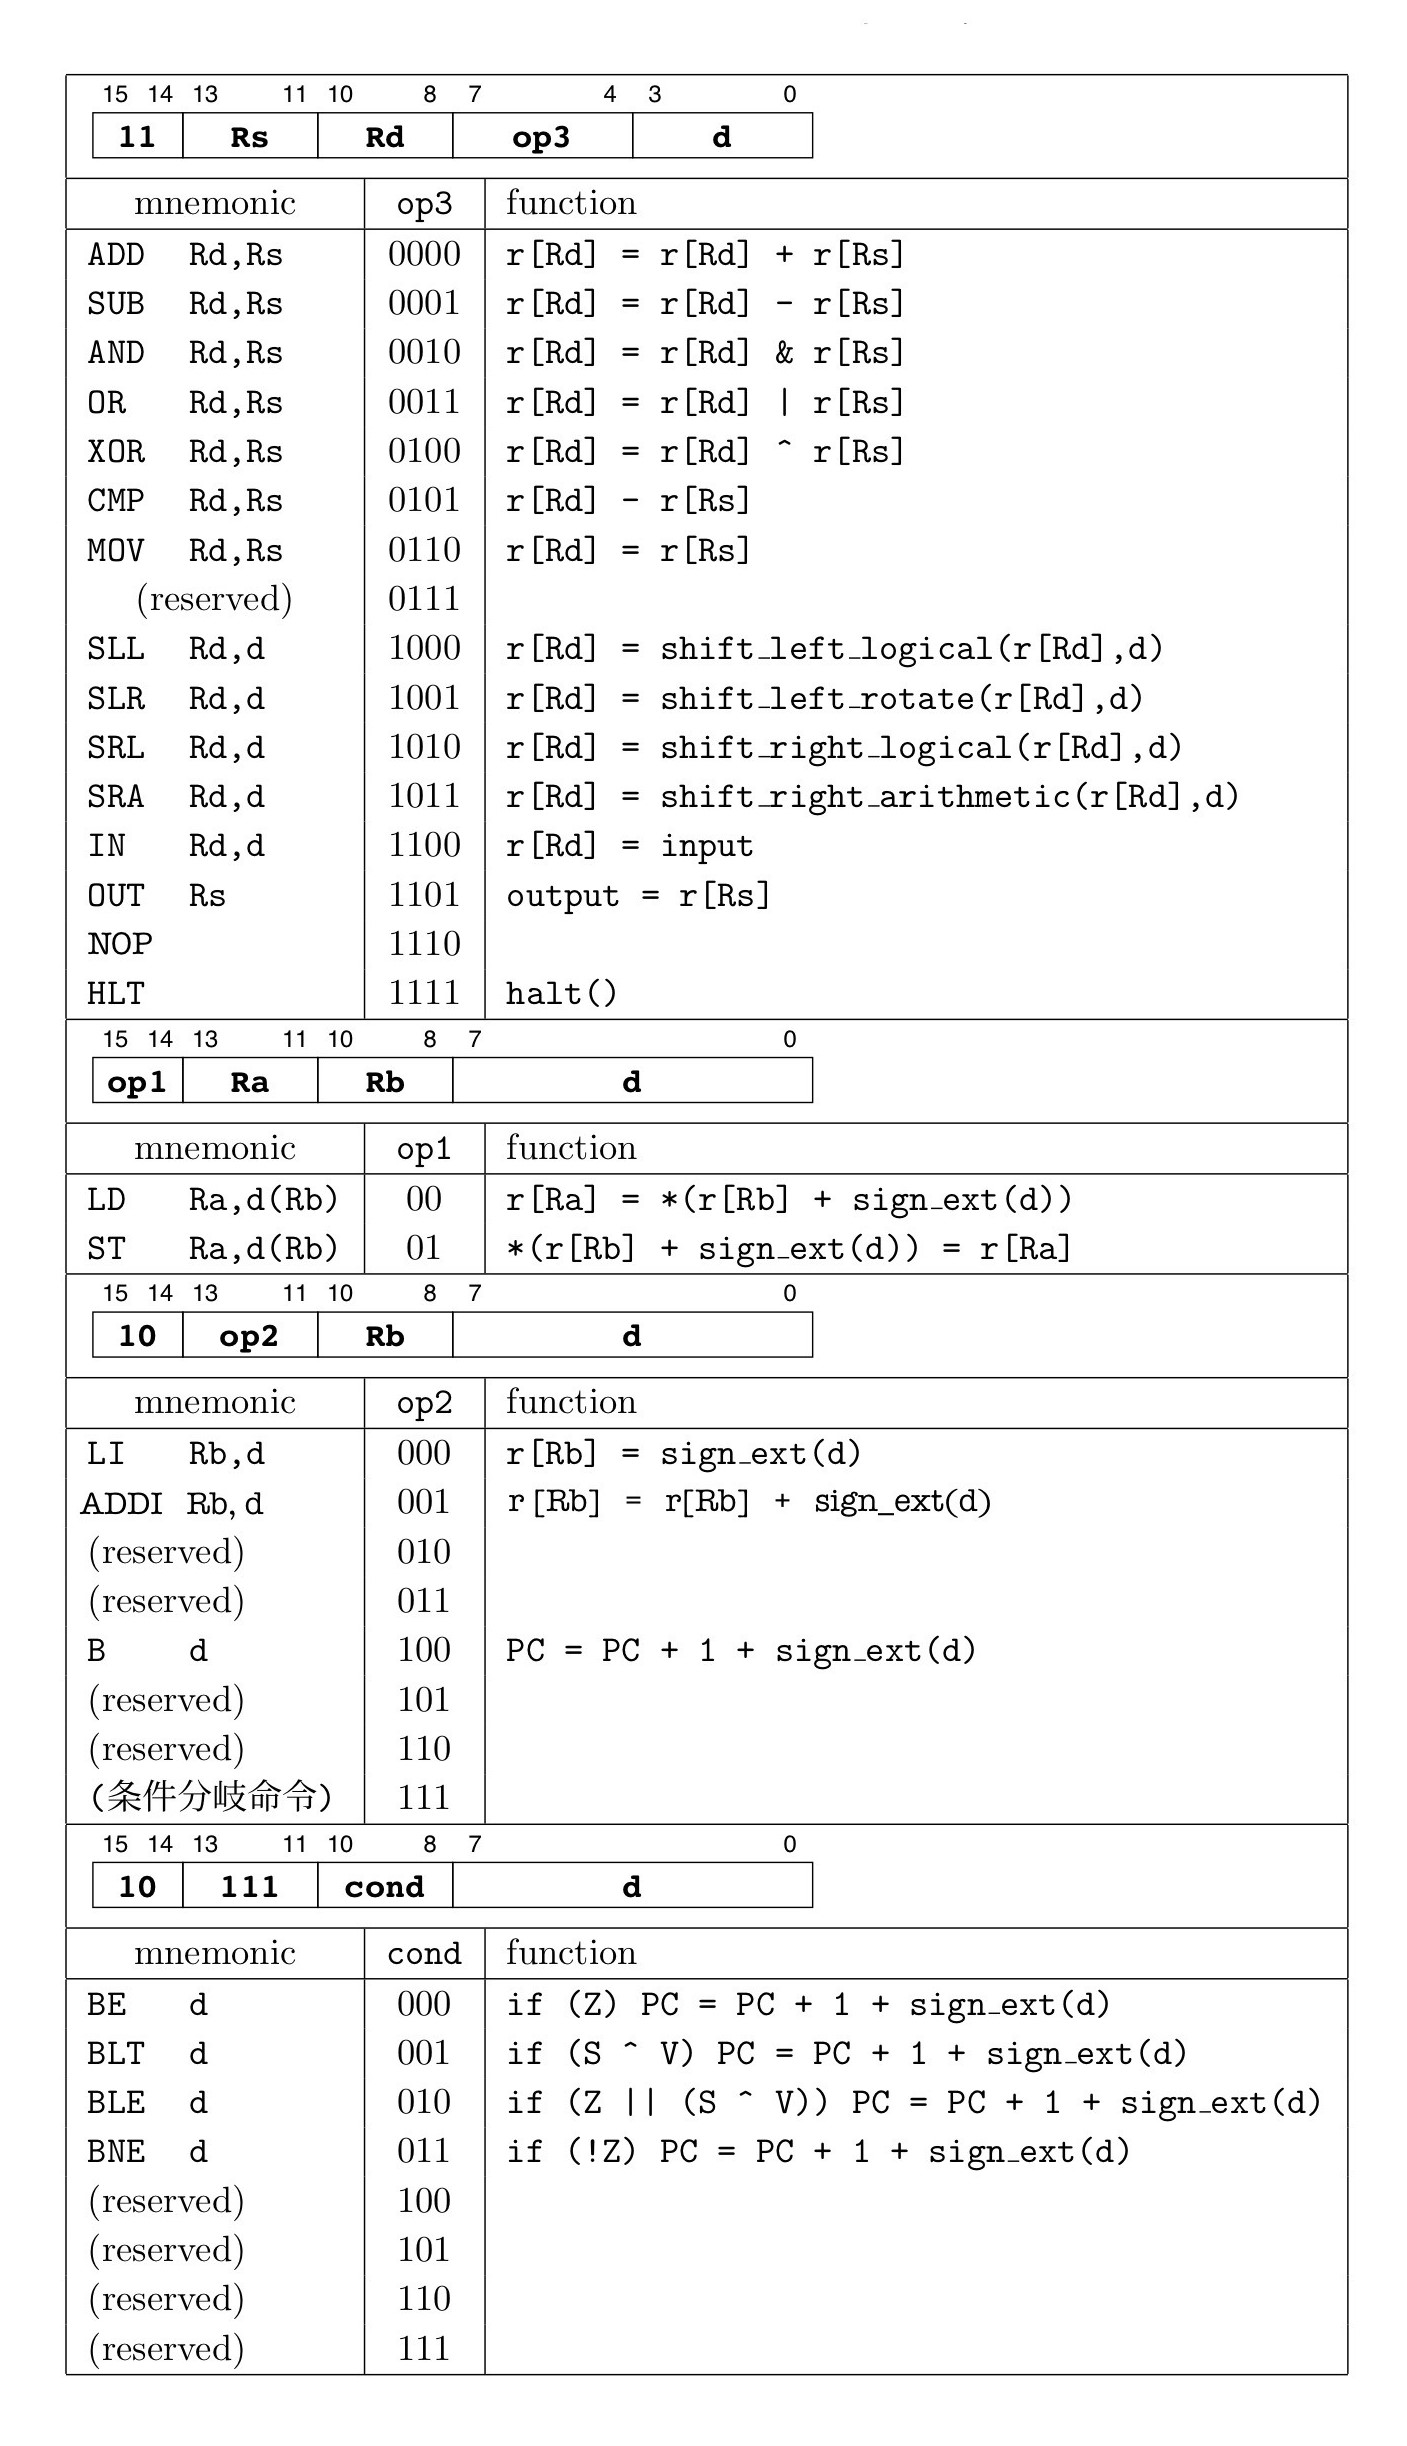
\includegraphics[scale = 0.22]{instructionSet.jpg}
    \end{center}
    \caption{命令セット・アーキテクチャ}
    \label{instructionSet}
\end{figure}

\subsection{IN命令}
IN命令が呼ばれると実行を一時的に中断し、外部入力で入力された値をうけとる。
中間発表の段階の外部入力では、実行の中断中に16個のディップスイッチを変更し、16bitの値を設定し、
execボタンを押すことでexecボタンが押された時のディップスイッチを用いて表現された値を入力として受け取り、
実行を再開するようにした。

\subsection{OUT命令}
OUT命令が呼ばれると、フェーズがp3の時に外部出力にRsフィールドで指定したレジスタの中身が渡される。
中間発表の段階の外部出力では7SEG-LEDを4つ用いて16進数表示で16bitのデータを表示する。
また、過去16回のOUT命令で出力されたデータを保持し、次のOUT命令が呼ばれるか、7SEG-LEDに表示し続ける。

\subsection{HLT命令}
命令の実行を中断するための命令である。内部的にはexecボタンが押されたのと同じ動作をする。
HLT命令が呼ばれた後に、execボタンを押すとメモリ上でHLT命令の次の命令から命令の実行を再開する。

\subsection{NOP命令(=non operation)}
レジスタ・メモリ書き込み、外部入出力などの動作を、何も行わない命令である。機器の初期化の際に、
resetボタンが押されるとInstruction Registerの値は2'b 1100000011100000となり、NOP命令の値に設定される。

\subsection{その他の命令}
ADD,SUB,AND,OR,XOR,CMP,MOV,SLL,SLR,SRL,SRA,LD,ST,LI,B,BE,BLT,BLE,BNEについては授業資料の命令セットの仕様通りに設計を行ったため、
授業資料の命令セットの説明と被る箇所は割愛する(授業資料のコピーを載せることになるので割愛)。
ただし、LD,ST,LI,IN,OUT命令でのSZCVのフラグについて、
それぞれの命令で移動するデータの値(LDならばメモリからロードするデータ、STならばメモリに格納するデータ、
LIならばレジスタに格納する即値の値、INならば入力として受け取るデータ、OUTならば出力するデータ)が、
正のときSZCV=0000、負のときSZCV=1000、0のときSZCV=0100となるようにSZCVフラグを設定した。


\section{構造と動作}



\end{document}